%%==================================================================%%
%% Author : Tejedo Gonz�lez, Daniel                                 %%
%%          S�nchez Barreiro, Pablo                                 %%
%% Version: 1.0, 10/12/2012                                         %%                   
%% Version: 2.0, 11/03/2013                                         %%                   
%%                                                                  %%
%% Memoria del Proyecto Fin de Carrera                              %%
%% semantica, pruebas                                              %%
%%==================================================================%%

Como ya se ha comentado, las pruebas relativas a la sem�ntica han de ser todo lo completas y exhaustivas que sea posible, pues engloban el funcionamiento completo de la aplicaci�n. Por lo tanto, en este punto hay que asegurarse que todos los componentes desempe�an la labor que les fue encomendada de manera correcta.

Para realizar esta bater�a de pruebas se ha llevado a cabo una t�cnica de caja negra. Esta estrategia se basa en intentar poner a prueba todos los conjuntos posibles de variables de entradas y salidas para todas y cada de una de las operaciones que nuestro software pueda llevar a cabo. 

\begin{figure}[!tb]
    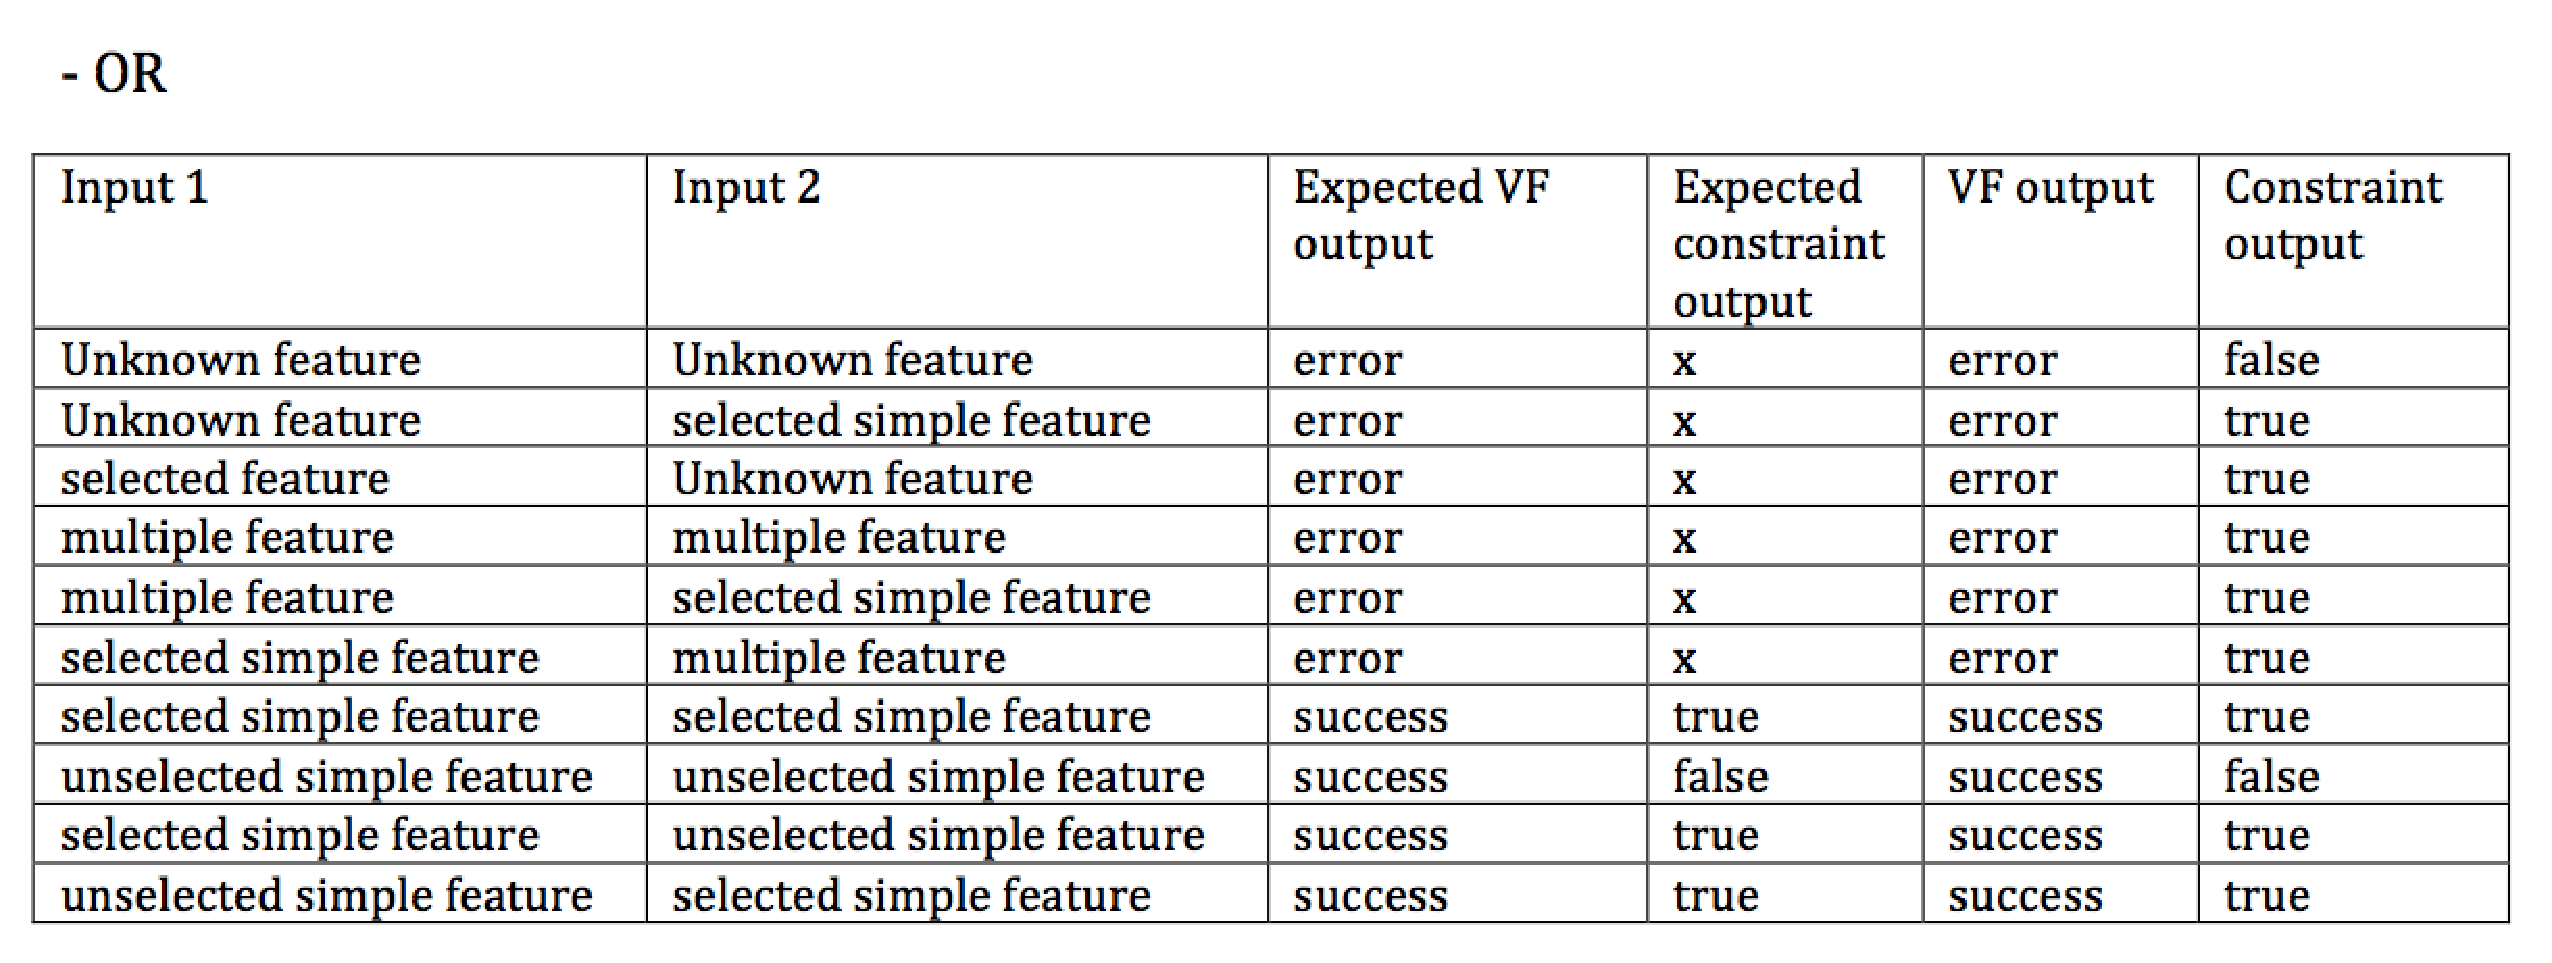
\includegraphics[scale=0.3]{semantica/pruebaOr.eps}
    \caption{Bater�a de pruebas para la operaci�n Or}
    \label{fig:pruebaOr}
\end{figure}


La Figura  muestra la tabla de pruebas llevadas a cabo para la operaci�n l�gica \emph{or}, as� como su resultado. Como se puede apreciar, tambi�n hemos aprovechado para realizar pruebas m�s exhaustivas de los mecanismos implementados mediante Validation Framework, ya que antes fueron imposibles de ser realizadas a este nivel de precisi�n. Una bater�a de pruebas similar a esta ha sido realizada para el resto de operaciones l�gicas, aritm�ticas y de comparaci�n.

Sin embargo, las operaciones de contexto no pueden ser sometidas a una tabla como la mostrada. Para probarlas, se han tenido en cuenta el n�mero de caracter�sticas que las operaciones \emph{all} y \emph{any} ten�an que comprobar, as� como el resultado esperado de la restricci�n o la presencia de contextos ternarios. En alg�n caso, las pruebas sirvieron para arreglar alg�n aspecto de la aplicaci�n que no hab�a sido implementada de modo apropiado.

El informe de pruebas es demasiado largo para ser incluido completo en ese informe. Se incluye el archivo \emph{pruebas.pdf} en el CD adjunto, en caso de querer ser consultado.